\chapter{Principy dnešního internetu věcí}
\label{ch:principy-iot}
Internet věcí lze z odborného hlediska klasifikovat jako síť fyzických zařízení komunikujících mezi sebou.
Primárním obsahem zpráv jsou hodnoty získané v koncových zařízeních a příkazy pro jejich interkaci se světem.
Data pro síť získává zařízení z okolního prostředí pomocí senzorů (nejčastěji neelektrických) veličin, přímé
uživatelské vstupy pomocí mechanických ovládacích prvků (tlačítka, přepínače, spínače), výstupy systému mohou být
realizovány pomocí zobrazovacích jednotek, signalizačních světel či reproduktorů, stejně tak jako pomocí motorů,
elektrických relé či krokových motorů.

Systémy pro Internet věcí lze v zásadě rozdělit dle vnitřní struktury na centralizované a decentralizované --
sítě centralizovaných systémů obsahují centrální prvek řídící okolní zařízení a nejčastěji i distribuující data mezi
nimi.
Decentralizované sítě jsou poté složeny pouze z množiny zařízení, u kterých dochází výhradně ke komunikaci mezi
samotnými uzly bez dodatečného prostředníka.
Porovnání základních vlastností těchto dvou konceptů lze nalézt v tabulce~\ref{table:iot-types}.

https://dzone.com/articles/the-internet-of-things-why-decentralization-must-b
\begin{table}
    \centering
    \caption{Srovnání vlastností základních koncepcí systému Internetu věcí.}
    \begin{tabularx}{\textwidth}{r|r|r}
        \, & \textbf{centralizovaný} & \textbf{decentralizovaný} \\
        \hline
        vliv selhání uzlu na síť & v případě centrálního uzlu fatální & absence pouze konkrétního uzlu \\
        \hline
        bezpečnost dat sítě & závislá na bezpečnosti centrálního uzlu & v případě použití blockchainu
        velmi vysoká~\cite{IoTeX} \\
        \hline
        zdroj pravdy v síti & centrální uzel & bez jednotného zdroje \\
        \hline
        konfigurace uzlů & z centrálního uzlu principem \uv{master-slave} & specifická pouze pro dotčené uzly \\
        \hline
        odolnost proti ztrátě dat & nižší vinou jednotného úložiště & vyšší v případě dat uložených v uzlech
    \end{tabularx}
    \label{table:iot-types}
\end{table}

\todo{Co je to IoT a proc jej potrebujeme?}
\blind{1}

\missingfigure{Schema centralizovaneho iot systemu}

\subsection*{Bezpečnost systémů}
\todo{Duraz na bezpecnost a uzivatelskou privetivost}
\blind{2}

\todo{Rozdelit na SW a HW casti}
\blind{1}

\section{Existující řešení}\label{sec:existujici-reseni}

Na realizaci systémů IoT se v dnešní době zaměřuje mnoho firem, stejně tak existuje několik variant s otevřeným kódem.
Často se jedná o kombinaci obou potřebných stránek pro provoz -- tedy, k hardwarovému řešení je poskytnuto i řešení
softwarové, ale existují i pouze jednostranné nástroje.
Dále budou představeni největší hráči na poli jak komerční sféry, tak sféry otevřeného zdrojového kódu.
\todo{citace https://chytrydumsvepomoci.cz/blog/vyber-systemu-pro-inteligentni-dum}

\subsection{OpenHAB -- open Home Automation Bus}\label{subsec:openhab}
OpenHAB je zástupcem softwarového řešení s otevřeným zdrojovým kódem v programovacím jazyce Java.
Díky tomu jej lze spustit prakticky na všech dostupných hardwarových řešeních\footnote{Jazyk Java pro svůj běh
používá JVM, což je prostředí obdobné k již zmíněnému Node.js, a které je schopno běhu na zařízeních založených nad
architekturami \textit{x86}, \textit{x86\_64}, \textit{ARM} a dalšími -- podpora architektury \textit{ARM} je
významná vzhledem k populárnímu mikropočítači Raspberry Pi, který je na ní založen.}.
Toto řešení nabízí možnost kompletní konfigurace serveru pro řízení IoT, jednotlivé uzly sítě mohou být k serveru
připojeny jak po síti Internet, tak lokálně např. pomocí rozhraní USB -- k rozšíření je dostupná obsáhlá
knihovna přídavných modulů.
OpenHAB je primárně založen na sestavení uživatelského rozhraní pro ovládání systému, ve kterém uživatel ovládá
připojená zařízení na základě pravidel, které mohou být nakonfigurována staticky či dynamicky pomocí dostupného
skriptování.

\subsection{Loxone -- Loxone Smart Home}\label{subsec:loxone}
Loxone je otevřený, avšak komerční systém nabízející jak hardwarové řešení, tak odpovídající softwarové řešení --
jádrem systému je miniserver s proprietárním programovou výbavou, která zajišťuje obsluhu pro karty tzv. \uv{Loxone
extension}, která jsou poté rozhraním pro komunikaci s okolním světem.

Toto řešení také nabízí experimentální funkci automatického naučení pravidel pro funkci celého systému, kdy
systém detekuje své vstupy a výstupy a na základě již existujících řešení vygeneruje pravidla.
Samotná manuální konfigurace je poté možná skrz nástroj Loxone Config, který zajišťuje zaslání požadované
konfigurace do miniserveru a nabízí i její lokální simulaci -- dvě takováto pravidla lze vidět na
obrázku~\ref{fig:iot-loxone-config}.

\begin{figure}%
    \centering
    % TODO: loxone from https://www.loxone.com/cscz/loxone-config-8
    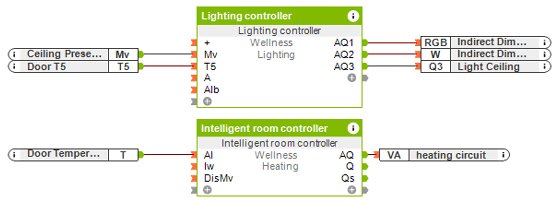
\includegraphics[width=\textwidth]{figures/iot-loxone-config.png}
    \caption{Detail z nástroje Loxone Config -- v levé části se nachází zařízení připojené do Loxone miniserveru
    figurující jako vstupy pro samotné pravidlo chování figurující uprostřed. %
    Vpravo jsou poté výstupy, pomocí kterých je rozhodnutí z pravidla aplikováno zpět do reálného světa.}
    \label{fig:iot-loxone-config}
    %
\end{figure}

\subsection{Domoticz}\label{subsec:domoticz}
http://www.domoticz.com/
https://doc.turris.cz/gadgets/domoticz
http://www.stehlikovi.eu/zapisky/raspberry-pi-z-wave-a-domoticz/

\subsection{Hardware}
\todo{Pro SW poresit Loxone/SmartHome}
\blind{1}

\subsection{Software}
\todo{Pro HW poresit komercni site/pyboardy a podobne}
\blind{1}

\section{ESP32}\label{sec:esp32}
\textit{ESP32} je řada nízkonákladových SoC\footnote{\textit{System on Chip} je integrovaný obvod obsahující veškeré
periferie (digitální, analogové a často i rádiová rozhraní) zabudované přímo v čipu.
Tento princip bývá použit ve vestavěných systémech díky jeho nízké spotřebě.} mikrokontrolérů představená čínskou
firmou Espressif Systems.
Jakožto nástupce řady \textit{ESP8266} nabízí na jediném čipu ve standardní distribuci následující:

\begin{itemize}
    \item dvoujádrový 32 bitový mikroprocesor Xtensa LX6, taktovaný na 160 či 240 MHz
    \item 520 KiB statické operační paměti
    \item Wi-Fi ve stadardu 802.11 b/g/n
    \item Bluetooth v4.2 včetně nízkoodběrového režimu BLE
    \item 12 bitový ADC až s 18 kanály
    \item dva 2 bitové DAC
    \item čtyři rozhraní SPI
    \item tři rozhraní UART
    \item deset GPIO pinů pro kapacitní použití
    \item rozhraní I\textsuperscript{2}C, I\textsuperscript{2}S, Hallovu sondu, sběrnici CAN, generátory PWM a další
\end{itemize}

\begin{figure}
    \centering
    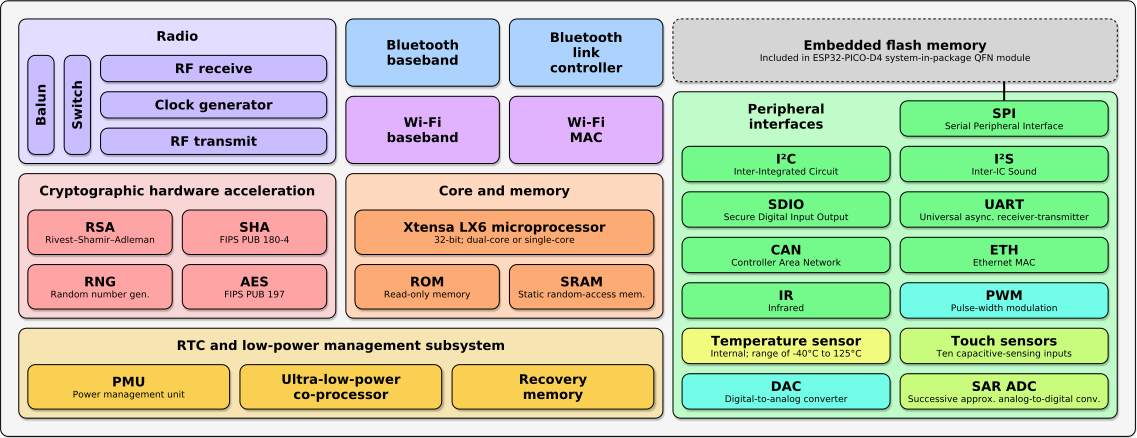
\includegraphics[width=\textwidth]{figures/esp-diagram.png}

    \caption{Diagram jednotlivých dostupných modulů na SoC ESP32 -- od jádra s procesorem a pamětmi obsahuje čip
    moduly pro bezdrátovou komunikaci, hardwarovou podporu kryptografie, podporu pro nízkoodběrový běh i periferie
    pro externí sběrnice.}

    \label{fig:esp-diagram}
    %\todo{obrazek z https://commons.wikimedia.org/wiki/File:Espressif_ESP32_Chip_Function_Block_Diagram.svg }
\end{figure}

Důležitou periférií je modul pro WiFi a Bluetooth komunikaci, který je obsluhován druhým jádrem procesoru.
Toto chování vyžaduje podporu od běžícího operačního systému, vzhledem k tomu, že je nutné přepínat kontext procesoru
právě pro správu připojení -- z tohoto principu kooperace jader bohužel plyne řada bugů v čipu, které vývojáři čipu
popsali v dokumentu \uv{ECO and Workarounds for Bugs}~\cite{ESP32KnownBugs}.
Pro část chyb existuje alternativní způsob, jak potlačit jejich dopad na standardní běh procesoru, stejně tak část
chyb byla vyřešena vydáním dalších revizí čipu ESP32.

Komunikace na WiFi protokolech využívá standardní model ISO/OSI, kdy na druhé, linkové vrstvě modul používá MAC
adresu, která je zabudována přímo v čipu při jeho výrobě\footnote{MAC adresa složená ze 48 bitů je na čipu
zaznamenána pomocí technologie eFuse.}.\todo{efuse}
Tato adresa je pro všechny vyrobené čipy ESP32 jedinečná a díky tomu, že je přístupná i pro uživatelskou programovou
výbavu, je možné i používat jako unikátní identifikátor jednotlivých čipů -- této vlastnosti bude využito při návrhu
protokolu dále v práci.

\begin{figure}
    \centering

    \subfloat[čip ESP32 integrovaný na vývojovém kitu ESP32 Devkit C]%
    {{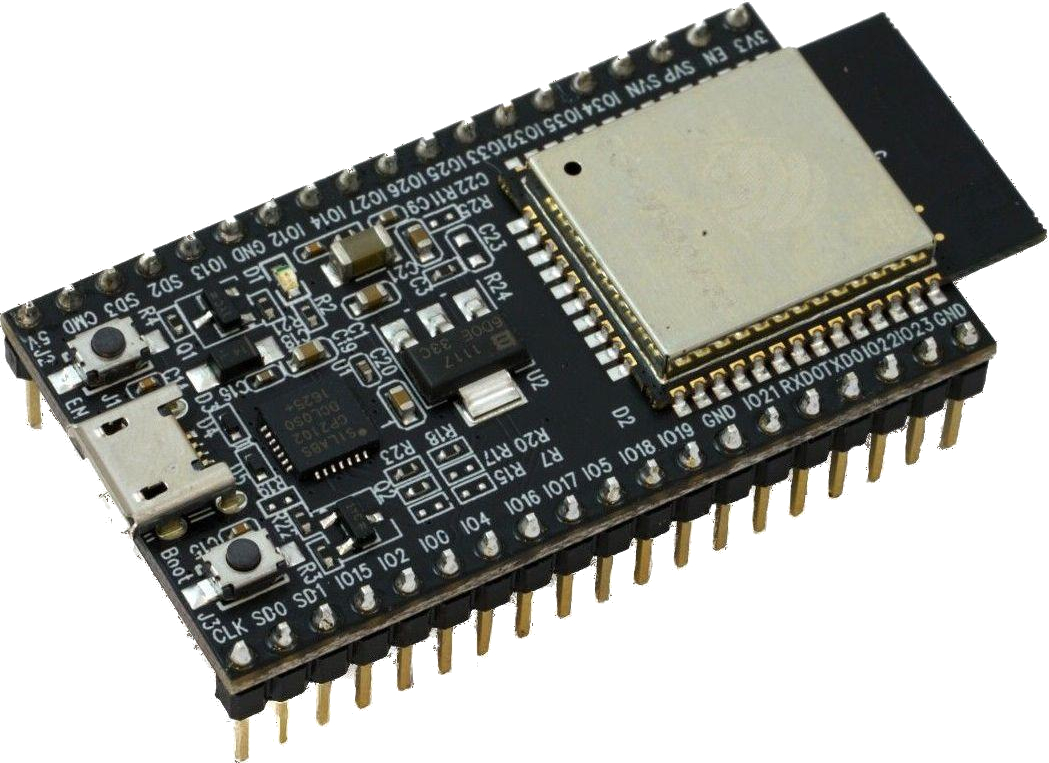
\includegraphics[valign=t,width=.35\textwidth]{figures/esp-devkitc.jpg}}}%
    \quad%
    \subfloat[samotný čip ESP32]%
    {{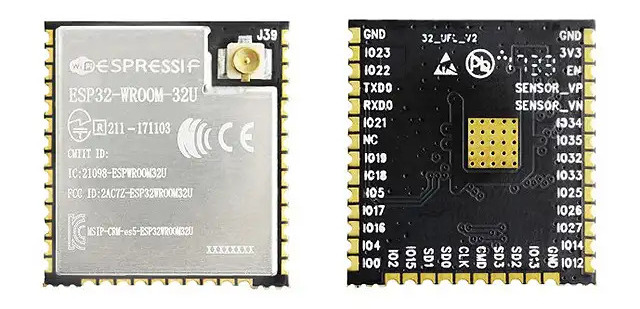
\includegraphics[valign=t,width=.6\textwidth]{figures/esp-chip.jpg}}}%

    \caption{Mikrokontrolér ESP32 je pro vývojové a výukové účely nejčastěji distribuován jako kompletní kit s USB
    konektorem pro napájení a vyvedenými piny z čipu. %
    Pro přímé aplikace je ovšem čip dostupný i ve své surové formě.}
    %\todo{z https://www.digikey.com/product-detail/en/espressif-systems/ESP32-WROOM-32U/1904-1026-1-ND/9381735}

    %\todo{z https://www.soselectronic.cz/products/espressif/esp32-devkitc-236729}
\end{figure}

\subsection{Měření neelektrických veličin}
\todo{Co vsechno se meri - kratky uvod do HW principu mereni?}
\blind{1}

\section{MicroPython}\label{sec:micropython}
MicroPython je derivátem vysokoúrovňového skriptovacího programovacího jazyka Python určený pro běh na vestavěných systémech a dalších
aplikacích s nízkým výpočetním výkonem.
Z hlediska vestavěné knihovny nabízí naprostou většinu základní knihovny z původní distribuce a navíc knihovny
zodpovědné za manipulaci s rozhraním mikropočítače, na kterém běží.
Kromě oficiálního sestavení pro pyboard\footnote{Oficiální (výukový) vývojový kit pro běh Micropythonu s
cenou okolo \pounds30 z oficiálního e-shopu.} nabízí komunita i sestavení pro ESP2866, ESP32, WiPy nebo Espruino Pico.

Sestavení pro kity od společnosti ESP jsou založena na vývojovém frameworku ESP-IDF.
Ten je zástupcem operačních systémů reálného času (RTOS), tedy systémů pro které je typické časové plánování jednotlivých úloh
a kritické jejich časově přesné spuštění -- to vše nzaložené na plánovači, který bývá napostradatelnou součástí.
ESP-IDF je konkrétně postaven nad FreeRTOS, který je de facto standardem a největším hráčem na poli RTOS s otevřeným
zdrojovým kódem. \todo{citace z https://www.simform.com/iot-rtos-selection/}
Jedním z benefitů tohoto typu systému je možnost použití programového řízení komunikačních rozhraní
(jako je SPI, I\textsuperscript{2}C nebo USART) -- tato rozhraní lze poté naimplementovat, není nutný konkrétní hardwarový prvek.

I přes omezenou vestavěnou knihovnu a vysokoúrovňovost tohoto jazyka jej lze použít ve světě internetu věcí --
a to i díky jeho paměťové optimalizaci.
Nespornou výhodou pro použití v internetu věcí je i dostupnost základních knihoven pro komunikaci s okolním světem.
MicroPython v základu nabízí knihovnu \ic{machine} s třídami \ic{Pin}, \ic{PWM} či \ic{ADC} --
každá z těchto tříd reprezentuje způsob, jak komunikovat s okolním světem pomocí vestavěných periférií
-- i vestavěná knihovna je ovšem svým obsahem závislá na konkrétní distribuci pro konkrétní vývojový kit.

Ústřední knihovnou pro pro komunikaci s okolím na vyšších vrstách poskytuje balíček \ic{network}, který zpřístupňuje
třídu \ic{WLAN}, která je zodpovědná za práci s modulem pro WiFi připojení a to jak v klientském módu, tak v módu
přístupového bodu.

\begin{code}[language=Python,caption={Ukázka práce }]
    import machine
    pin = machine.Pin(14, mode=machine.Pin.OUT)
    pin.value(1)
\end{code}


\section{Message Queuing Telemetry Transport}\label{sec:mqtt}
Message Queuing Telemetry Transport (MQTT) je protokol definovaný ISO standardem určený pro kanálovou komunikaci zařízení
mezi sebou.
Jedná se o typ komunikace klient-server nad protokolem TCP/IP, server je dle svých vlastností nazýván specificky jako \uv{broker}.
Klient má možnost si po připojení zaregistrovat odběry jednotlivých kanálů -- jejich identifikace má tvar
alfanumerických řetězců oddělených pomocí znaku \ic{/}.
Benefitem přístupu s jasně definovaným oddělovačem je možnost použití zástupných znaků pro
zaregistrování odběru více kanálů zároveň.
Této vlastnosti bude využito v pozdější části práce pro komunikaci s uzly.
Znak \ic{+} je použit pro zastoupení jedné úrovně kanálu, znak \ic{#} pro víceúrovňové zahrnutí -- demonstrace těchto
principů je shrnuta v tabulce~\ref{table:mqtt-subscribes}.

V následujících podkapitolách budou popsány specifické vlastnosti protokolu MQTT důležité pro další postup v této
práci.

\subsection{Příznak zprávy \uv{retain}}\label{subsec:priznak-zpravy-retain}
Pomocí příznaku \uv{retain} může klient pro zprávu v konkrétním kanálu zažádat o její ponechání v kanálu pro budoucí
klienty -- tedy, zaregistruje-li si klient kanál k odběru, broker klientovi automaticky po zaregistrovásíní odešle
zprávy,
spadající tohoto kanálu (či kanálů v případě zástupných znaků), které mají nastavený tento příznak.

Tohoto chování lze velmi dobře využít pro kanály obsahující stav kterékoliv části ze systému --
nově připojený klient pak ihned dostane zprávu o stavu a nedochází k časovému intervalu, kdy je sice klient
zaregistrovaný, ale teprve čeká na novou aktualizaci stavu.

\subsection{Quality of Service}\label{subsec:quality-of-service}
Quality of Service (QoS) je pro MQTT vlastnost stanovující, k jak důslednému potvrzování zpráv by mělo mezi
brokerem a klientem docházet.
Ve své podstatě stanovuje, ke kolika potvrzení odeslané zprávy musí dojít, aby byla
zpráva prohlášena za úspěšně odeslanou.
Na obrázku~\ref{fig:mqtt-qos} jsou znázorněny směry zpráv protokolu mezi odesílatelem a příjemcem pro jednotlivé
hodnoty dostupné pro QoS:

\begin{enumerate}
    \item[\textbf{0}] U zprávy nedochází k potvrzování, je odeslána a je na ni zapomenuto.
    \item[\textbf{1}] Pro zprávu je zasláno od příjemce jedno potvrzení, je tedy zajištěno alespoň jedno doručení.
    \item[\textbf{2}] Kromě zpětného potvrzení je potvrzeno i samotné první zpětné potvrzení, příjemce tedy
    odesílateli potvrdí příjetí a smazání ze svého úložiště -- zpráva poté není distribuována vícenásobně.
\end{enumerate}

\begin{figure}
    \centering
    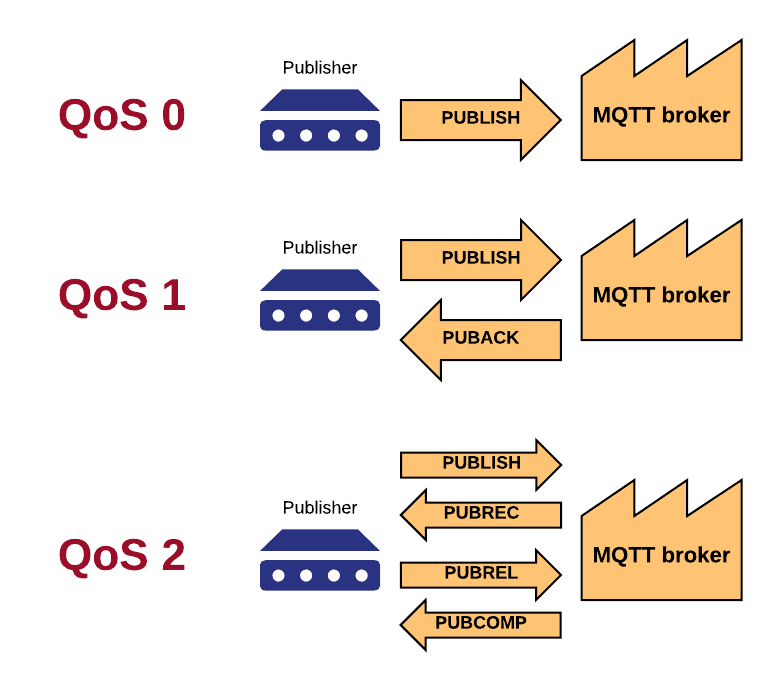
\includegraphics[width=.5\textwidth]{figures/mqtt-qos.png}
    \caption{Tři typy QoS pro MQTT - $0$ pro zprávy bez potvrzování (doručení nejvýše jednou), $1$ pro jednosměrné
    potvrzení (doručení alespoň jednou) a $2$ pro obousměrné potvrzení (doručení právě jednou).}
    \label{fig:mqtt-qos}
    %\todo{obrazek z ROOT.cz https://i.iinfo.cz/images/116/bigclown-2-3-prev.png }
\end{figure}

\subsection{Identifikace klienta \uv{Client ID}}\label{subsec:identifikace-klienta-client-id}
Možností klienta je zapsat si při připojení k brokeru své \uv{Client ID}.
Jedná se o řetězec jednoznačně identifikující konkrétního klienta -- hlavním benefitem je (v případě podpory
persistentních sezení) je možnost zachování zaregistrovaných kanálů k odběru v případě odpojení a
opětovného připojení klienta a také uschování prozatím nedoručených zpráv s QoS nastaveným na hodnotu 1 či 2.

Klient tedy zahájí komunikaci zprávou \ic{CONNECT}, která kromě dalšího obsahuje parametry \uv{Client ID} a \uv{Clean
session} -- druhý zmíněný vynucuje vyčištění sezení (smazání odběru a čekajících zpráv).
Broker poté odpovídá pomocí zprávy \ic{CONNACK}, která obsahuje informaci o úspěšnosti připojení a stavu sezení (zda
bylo vyčištěno či se podařilo připojit do existujícího).

\subsection{Parametr spojení \uv{Keep Alive}}\label{subsec:parametr-spojeni-keep-alive}
Parametr \uv{Keep Alive} určuje časový interval, během kterého musí klient odpovědět na zprávu \ic{PINGREQ} zprávou
\ic{PINGRESP} -- jestliže se tak nestane, spojení je ukončeno.
Tento parametr je nutný kvůli nežádoucí vlastnosti protokolu TCP --
v tomto protokolu, nad kterým je MQTT založen, může dojít k situaci tzv. polootevřeného spojení.

Je to standardně nežádoucí stav, při kterém je jedna ze stran spojení informována o ukončení spojení (jakoukoliv
vinou), druhá však ne.
To vede k čekání na potvrzení odeslaných zpráv na druhé straně, která ovšem nepřichází -- MQTT spojení se poté
tváří jako otevřené, ale není tomu tak.

\subsection{\uv{Last Will} zpráva}\label{subsec:last-will-zprava}
Zpráva s tímto příznakem je klientem nastavena při připojení k brokeru a brokerem je použita ve chvíli, kdy dojde
k neočekávanému odpojení klienta.
Tato zpráva \uv{poslední vůle} kromě samotného obsahu u sebe nese i cílový kanál, QoS či \uv{retain}
příznak.
MQTT tímto nabízí možnost klientům informovat o svém stavu odpojení autonomně bez dalšího zásahu --
\uv{Last Will} zpráva je odeslána do daného kanálu v následujících případech:
\begin{itemize}
    \item Klient neodpoví ve smluveném intervalu \uv{Keep Alive}.
    \item Klient před ukončením spojení neodešle zprávu protokolu \ic{DISCONNECT}.
    \item Broker ukončí spojení vinou chyby samotného protokolu.
    \item Broker detekuje IO chybu nebo chybu sítě.
\end{itemize}

\begin{table}
    \centering
    \caption{Možnosti odběru zpráv v protokolu MQTT -- používají se dva typy zástupných znaků pro zaregistrování
    odběru více kanálů naráz.}
    \begin{tabularx}{\textwidth}{ssr}
        \textbf{kanál zaregistrovaný k odběru} & \textbf{kanál zprávy} & \textbf{bude zpráva zahrnuta?} \\
        \hline
        \ic{node/1}
        &
        \texttt{node/1} \newline
        \texttt{node} \newline
        \texttt{node/1/status} \newline
        \texttt{node/2}
        &
        \truemark \newline
        \falsemark \newline
        \falsemark \newline
        \falsemark
        \\

        \hline
        \ic{node/+/status}
        &
        \texttt{node/1/status} \newline
        \texttt{node/2/status} \newline
        \texttt{node/foo/status} \newline
        \texttt{node/1/data} \newline
        \texttt{node} \newline
        \texttt{node/2}
        &
        \truemark \newline
        \truemark \newline
        \truemark \newline
        \falsemark \newline
        \falsemark \newline
        \falsemark
        \\

        \hline
        \ic{node/\#}
        &
        \texttt{node/1} \newline
        \texttt{node/2/status} \newline
        \texttt{node/2/status/data} \newline
        \texttt{node/} \newline
        \texttt{block/}
        &
        \truemark \newline
        \truemark \newline
        \truemark \newline
        \falsemark \newline
        \falsemark
        \\

        \hline
        \ic{node/+/data/\#}
        &
        \texttt{node/1/data/value} \newline
        \texttt{node/2/data/value/degrees} \newline
        \texttt{node/1/data/value} \newline
        \texttt{node/1/status/value} \newline
        \texttt{node/} \newline
        \texttt{block/}
        &
        \truemark \newline
        \truemark \newline
        \truemark \newline
        \falsemark \newline
        \falsemark \newline
        \falsemark
        \\

    \end{tabularx}
    \label{table:mqtt-subscribes}
\end{table}
